\subsection{Reference- and Validation Point Compositions}

\subsubsection{Number of Reference Points}
Basically, selecting four reference point pairs is enough to calculate a 
homography matrix $\mathrm{H}$. However, real-world measurements introduce 
noise. Accordingly, we can use optimization techniques and more point 
pairs to estimate $\mathrm{H}$, resulting in an overdetermined system of 
linear equations. By using more points, we can consider more scene 
characteristics. 

\begin{figure}
	\centering
		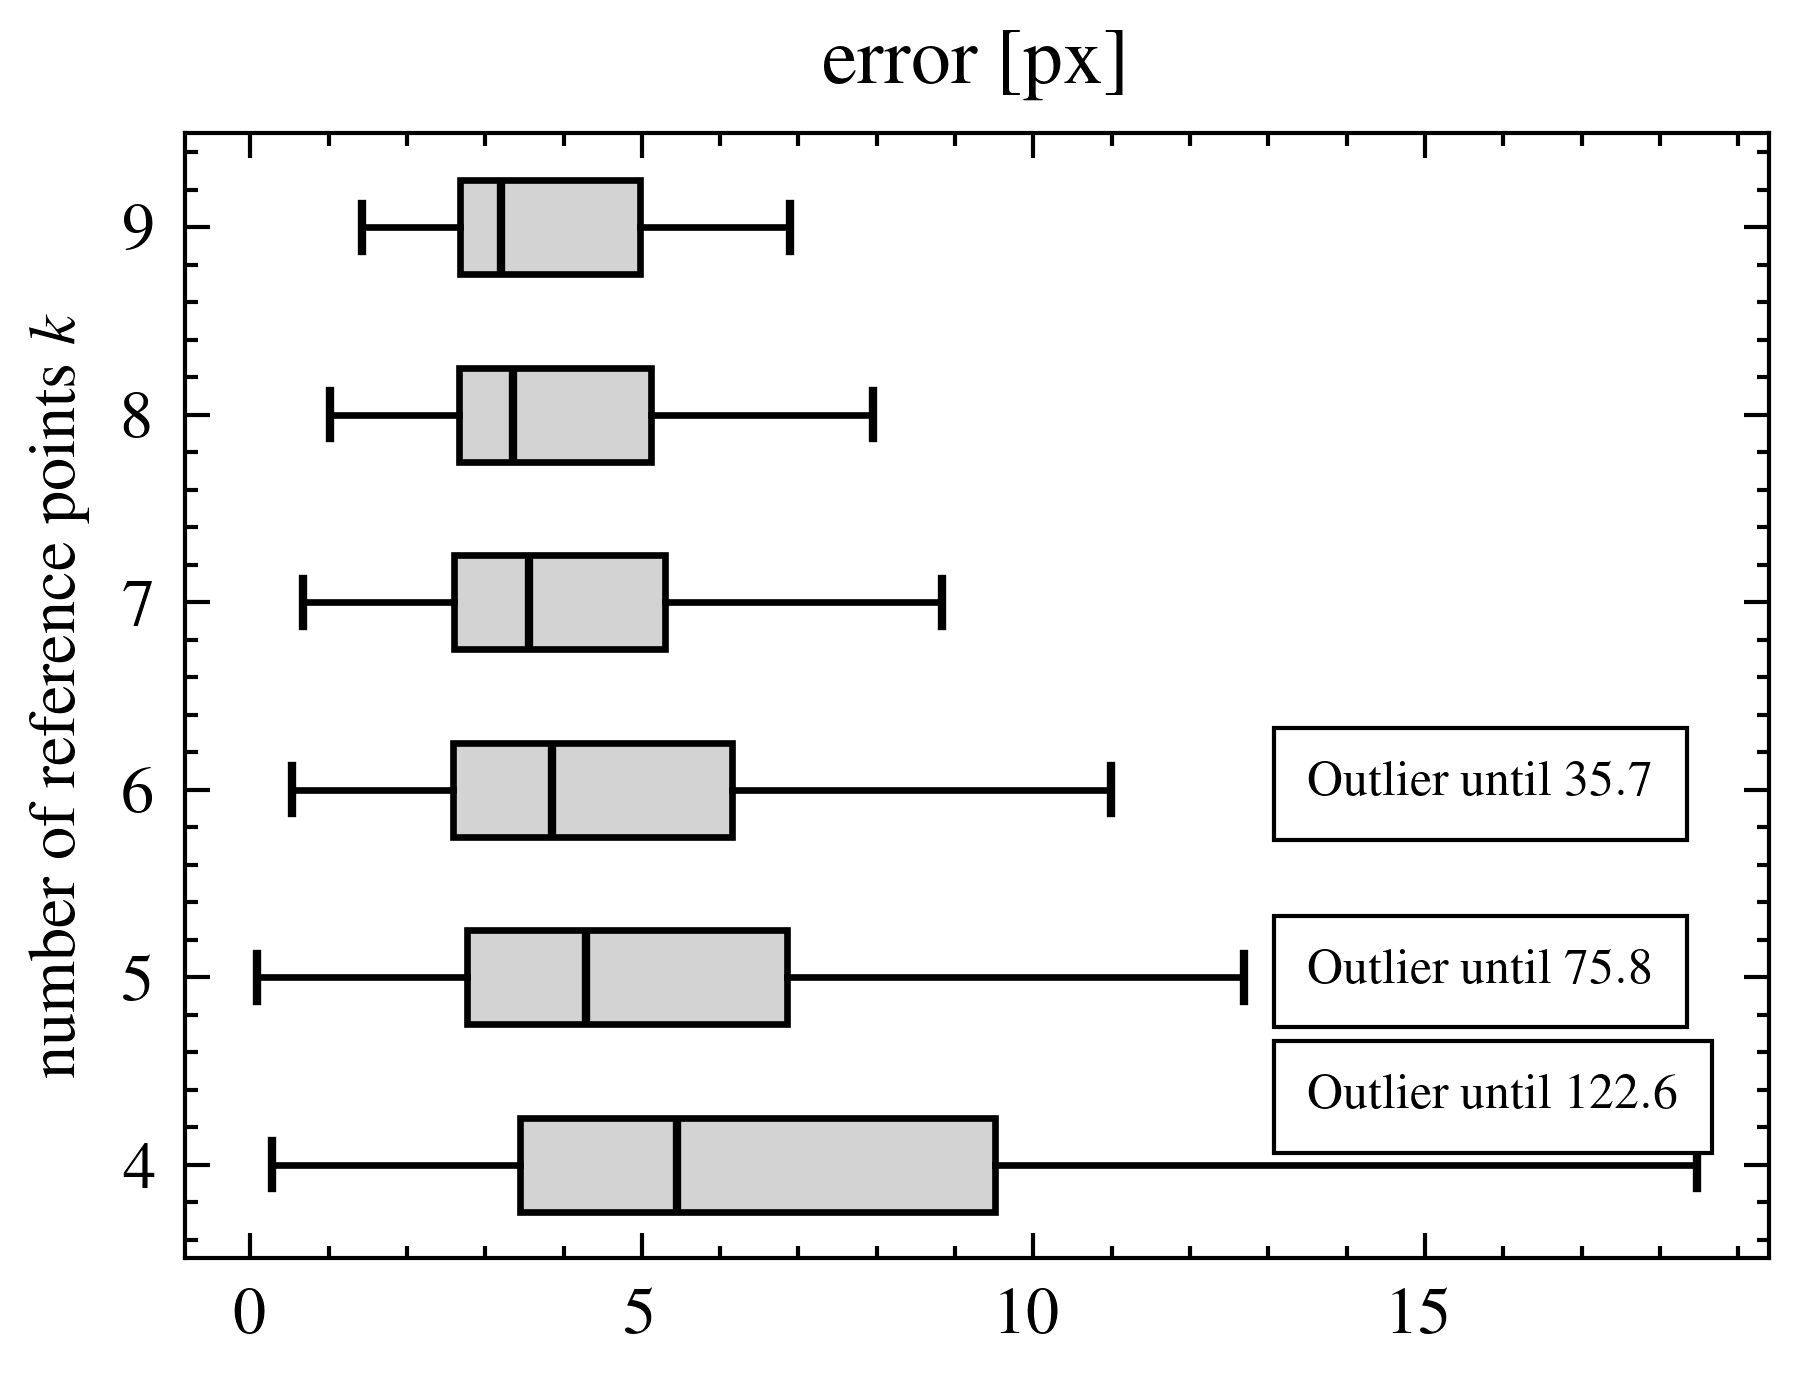
\includegraphics[width=0.45\textwidth]{figures/boxplot_errors_by_k_filtered.png}
	\caption{We chose all possible subsets of $k$ reference points and 
	calculated the error for each of the six validation points in IMG\_01 
	for each subset. Hence, we excluded all homographies with a 
	collinearity score of $< 1$.}
	\label{fig:boxplot_error_by_k_filtered}
\end{figure}

To determine the minimal number of points to be used, we analyze IMG\_01 
in more detail. The image contains nine reference points and six validation 
points, respectively. Previously, we used all reference points to calculate 
the corresponding homography matrix $\mathrm{H}_{01}$ and estimated the 
average error for all validation points, i.e., $6.95$ cm. 

In contrast to our earlier experiments, we use every possible composition 
of at least four reference points to determine $\mathrm{H}_{01}$ and estimate 
the average error. Hence, we conduct $382$ experiments for IMG\_01, 
consisting of the following point combinations, where $k$ denotes the number 
of used reference points to calculate $\mathrm{H}_{01}^i$, with 
$i \in \{ 1, 2, ..., 382 \}$:
\begin{align*}
	k=4 \rightarrow 126, k=5 \rightarrow 126, k=6 \rightarrow 84, \\
	k=7 \rightarrow 36, k=8 \rightarrow 9, k=9 \rightarrow 1.	
\end{align*}
Note that every single experiment calculates the errors for each 
validation point. Hence, the resulting dataset consists of $382 * 6 = 2.292$ 
data points.

Our random choice of reference points influences the homography matrix 
$\mathrm{H}_{01}^i$ and the quality of our reference, and validation points.
Using all nine reference points makes the homography less prone to 
degeneracy due to collinearity, validation points tend to be closer to 
reference points, etc. We will discuss those effects in detail subsequently. 
However, we exclude some point compositions with high collinearities
for our first, overall comparison to eliminate some significant outliers 
when only using four reference points.

Figure \ref{fig:boxplot_error_by_k_filtered} summarizes the results and implies that 
four reference points might be sufficient\textemdash but their composition is
crucial, even when neglecting collinearities.
With additional points, we may increase our confidence in obtaining
an accurate outcome. 


\subsubsection{Reference Point Compositions}
The choice of reference points enormously impacts a homography's quality. 
We have determined four factors for further investigation.

\paragraph{Collinearity}
To determine $\mathrm{H}_{01}$, we need at least four point pairs, i.e., 
we use $k=4$ reference points. However, the 
calculation collapses when at least three points are collinear. 
Nevertheless, collinearity rarely exists in 
real-world scenarios. Our experiments show that if three points are almost 
collinear, homographies still collapse. In the following, we will call those 
points collinear, even if, mathematically, they are not. 
IMG\_01 has three obvious collinear points: $w_4$, $w_5$, and $w_7$; 
calculating the homography with any other point produces degenerate 
solutions with intolerable errors. 

\begin{figure}
	\begin{center}
		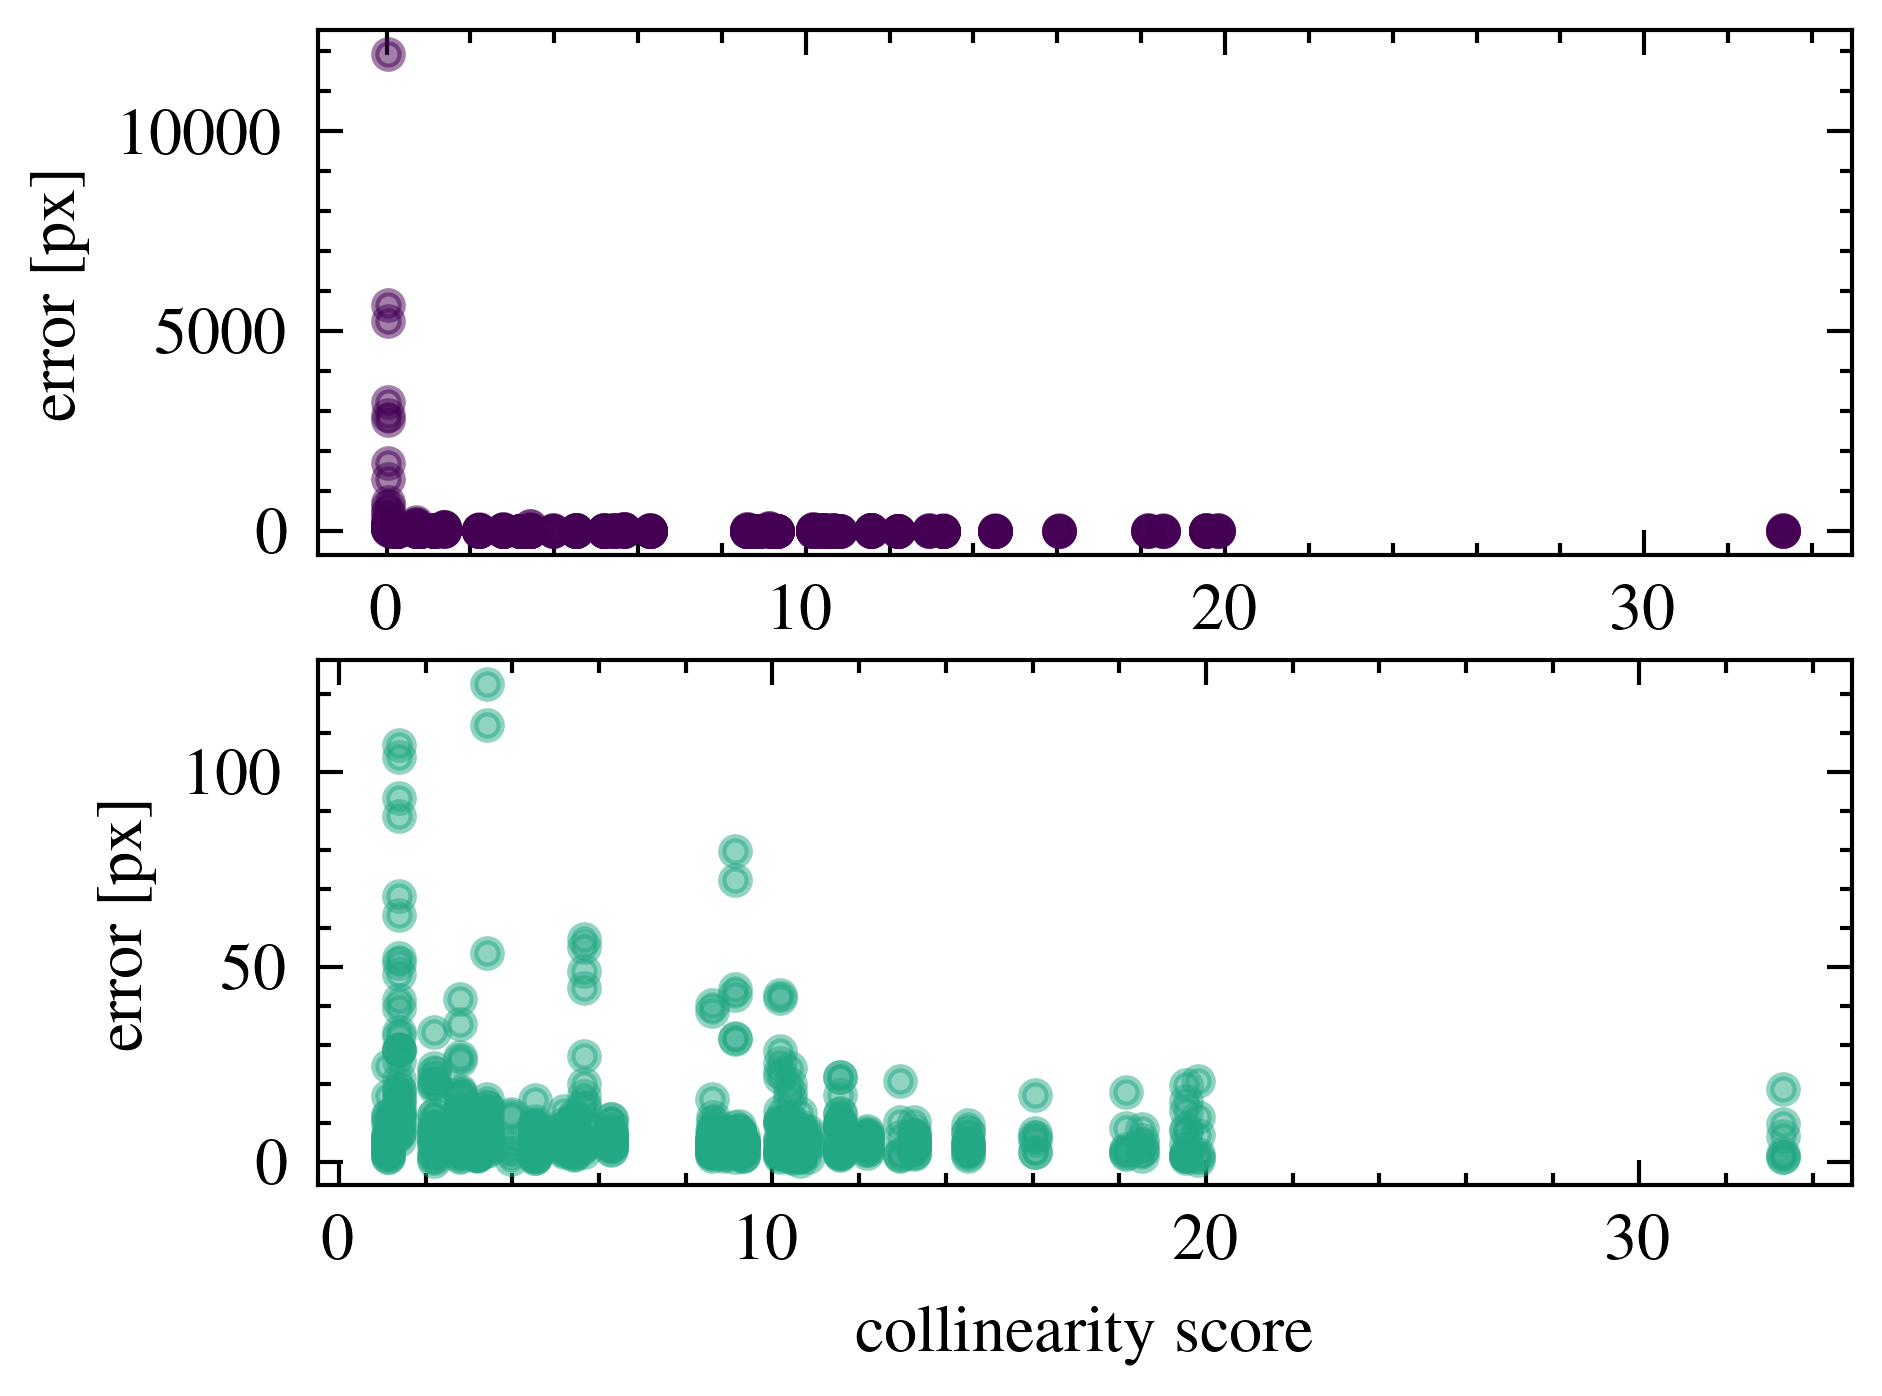
\includegraphics[width=0.45\textwidth]{figures/collinearity_error.png}
	\end{center}
	\caption{The error w.r.t. the collinearity scores (image above). The 
	error reduces significantly when excluding collinearity scores of 
	less than one (image below).}
	\label{fig:collinearity_error}
\end{figure}

However, $w_4$, $w_5$, and $w_7$ are not the only three collinear points. 
We propose to use the 
triangle inequality to determine collinearity. Given three reference points 
$w_i$, $w_j$, and $w_k$, and their corresponding edges $x$, $y$, and $z$, 
we calculate the collinearity $c(w_i, w_j, w_k)$ as follows:
\begin{equation}
\begin{aligned}
c(w_i, w_j, w_k) = \frac{x + y - z}{z},
\end{aligned}
\end{equation}
where $x,y,z\neq0$, $z > x$, and $z > y$. Because of the triangle inequality 
$z \geq x + y$. If three points lie within 
one line $c(w_i, w_j, w_k) = 0$. 
Note that a lower value corresponds to a higher collinearity.
For IMG\_01, this results in the collinearity values shown in 
Table \ref{tab:collinearity_values}.

\begin{table}[ht]
	\caption{Collinearity Scores for IMG\_01}\label{tab:collinearity_scores}
\begin{tabular*}{\columnwidth}{@{\extracolsep{\fill}} @{\hspace{40pt}}l r@{\hspace{40pt}}}
			\toprule
			\textbf{Reference Points} & 
			\textbf{Collinearity Value} \\
			\midrule
			w4, w5, w7 & 0.03 \\
			w5, w6, w9 & 0.12 \\
			w5, w6, w22 & 0.25 \\
			w4, w6, w21 & 0.69 \\
			w4, w8, w9 & 0.79 \\
			w4, w6, w22 & 1.12 \\
			... & ... \\
			w4, w6, w7 & 98.04 \\
			\bottomrule
		\end{tabular*}
	\label{tab:collinearity_values}
\end{table}

% \begin{figure}
	% \begin{center}
		% 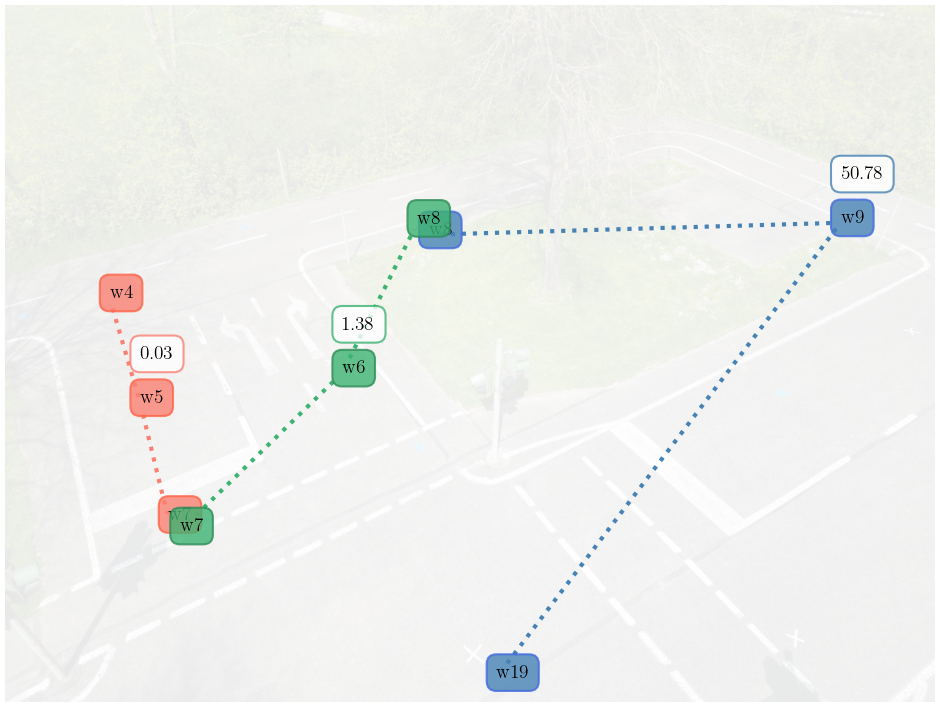
\includegraphics[width=0.35\textwidth]{figures/collinearity_examples.png}
	% \end{center}
	% \caption{This figure demonstrates three different collinearity values. 
		% When three reference points lie on the same line, the collinearity 
		% value approaches zero.}
		% \label{fig:collinearity_examples}
% \end{figure}

Each Homography $\mathrm{H}_{01}^i$, with $i \in \{ 1, 2, ..., 126 \}$ 
obtains $\begin{pmatrix} 4 \\ 3 \end{pmatrix} = 4$ collinearity values $c_1^i, c_2^i, c_3^i, c_4^i$.
If at least one subset is collinear, the homography collapses. 
Thus, we can take the smallest collinearity value to obtain the 
final collinearity score for $\mathrm{H}_{01}^i$:
\begin{equation}
\begin{aligned}
	c(\mathrm{H}_{01}^i) := \min{(c_1^i, c_2^i, c_3^i, c_4^i)}
\end{aligned}
\end{equation}

Thus, we can conduct the 126 experiments by selecting all reference point 
combinations within IMG\_01, where $k=4$. Every experiment produces 
six measurements. Figure \ref{fig:collinearity_error} shows the 
impact of collinearity. When excluding the twenty-nine homographies with a 
collinearity score of less than one, the error reduces drastically. 
We can improve a homography's robustness against collinearity by 
increasing the number of reference points $k$.

\paragraph{Distance to Next Reference Point}
The homography assumes that all points lie on the same plane ($Z=0$). The 
more we violate this assumption, the less precise our predictions are. 
Close points tend to have similar $Z$ coordinates generally. Suppose a 
validation point is close to a reference point: The $Z$ coordinate should be 
similar, and the error will be low, as we fitted the homography to 
this exact point.

However, suppose we used more than four points to calculate $\mathrm{H}$. 
Then, using optimization techniques, the argument loses some soundness. 
Nevertheless, the information is still being used and should be 
(on average) better than when no reference points are nearby.

\paragraph{Spanned Area}
Spanning larger areas entails considering more scene characteristics, 
correlating with the distance to the next reference points. 
Figure \ref{fig:error_by_area_and_distance} shows the impact of the 
spanned area and the validation point's distance to the next 
reference point, using the data from our collinearity experiments.
Large areas and close reference points decrease the 
errors by reducing the number of outliers.

\begin{figure}
	\begin{center}
		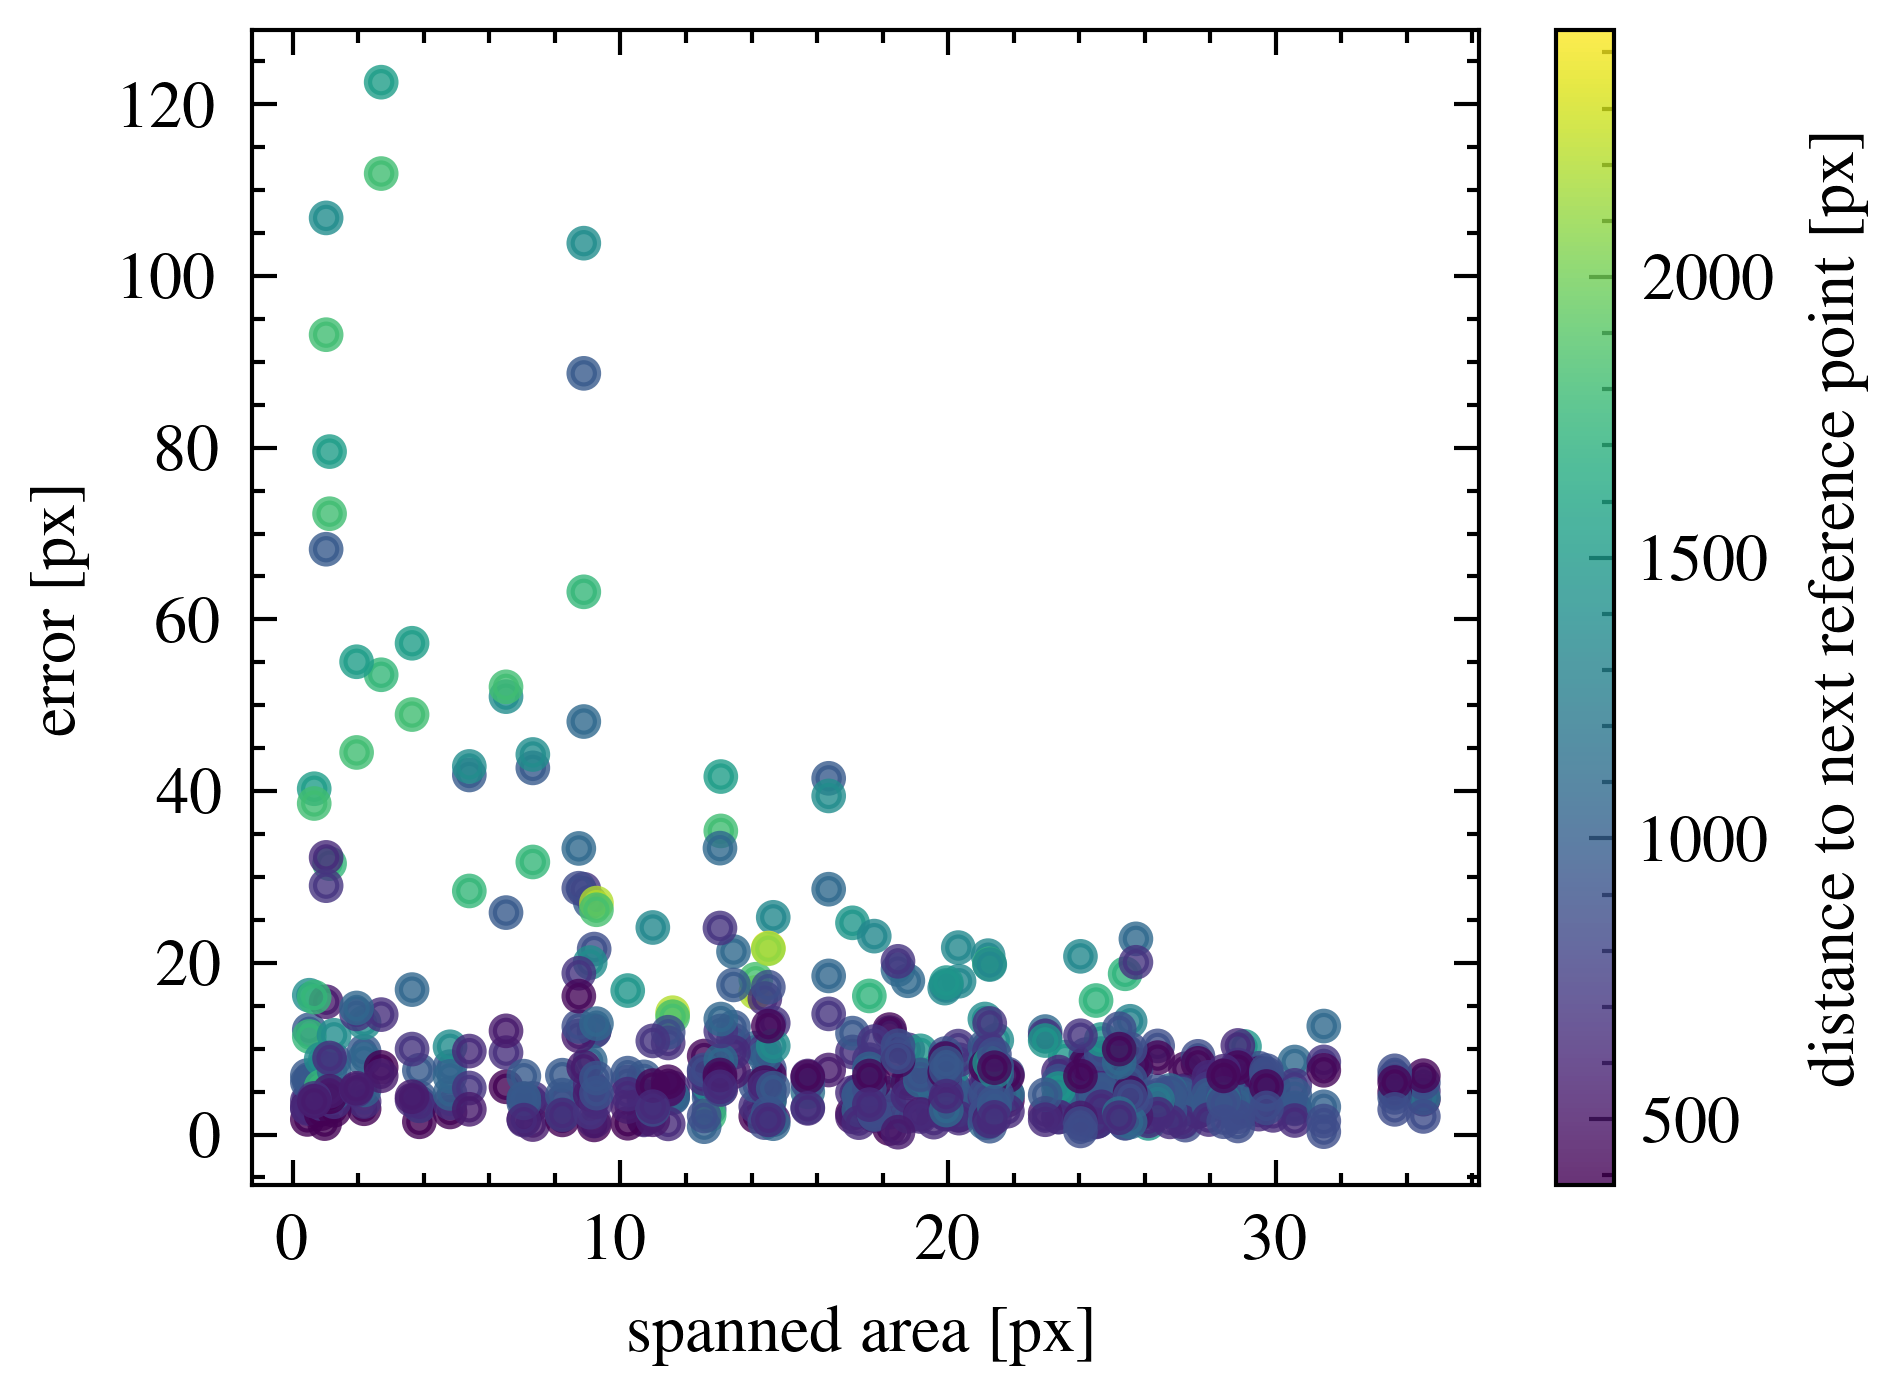
\includegraphics[width=0.45\textwidth]{figures/scatter_error_by_area_distance.png}
	\end{center}
	\caption{The error with respect to the spanned area and the distance
	to the next reference point, after excluding homographies with 
	a collinearity score of $c < 1$.}
	\label{fig:error_by_area_and_distance}
\end{figure}

\paragraph{Pixel Density}
The closer the validation point to the camera, the more pixels encircle it. 
A higher number of surrounding pixels results in a better prediction because 
the random noise within the perspective view loses its impact.

We propose to quantify a validation point's pixel density as follows: 
Imagine four points surrounding the validation point in the top view, each 
located $n$ pixels away in the $x$, $-x$, $y$, and $-y$ directions. 
Transform these four surrounding points into the perspective view using the 
inverse homography $\mathrm{H}^{-1}$. Now, to measure pixel density, 
calculate the average distance between these surrounding points and the 
validation point within the perspective view. A higher pixel density 
indicates more pixels available around the validation point in the 
perspective view.

To test our hypothesis about better predictions with high pixel densities 
due to random noise losing its impact, we select two similar validation 
points, $b_{8}$ and $b_{21}$. Using the four reference points $w_6$, $w_8$, $w_9$, 
and $w_{22}$, we ensure that the distance to the nearest reference 
points remains similar. 
Then, we calculate the error for each point. Additionally, we apply 
random Gaussian noise to the reference points with a standard deviation 
increasing by five pixels up to 70. We repeat the process 100 times for each 
standard deviation and compute the average. Figure \ref{fig:density} 
presents the average error. The validation point with a higher pixel density seems more 
resistant to the noise, and the error grows more slowly. We repeated the 
process also for IMG\_02 with the reference points 
$w_{21}, w_{23}, w_{26}, w_{28}$ and validation points $b_{24}, b_{28}$ and 
the same behavior has been observed. 

\begin{figure}
    \centering
        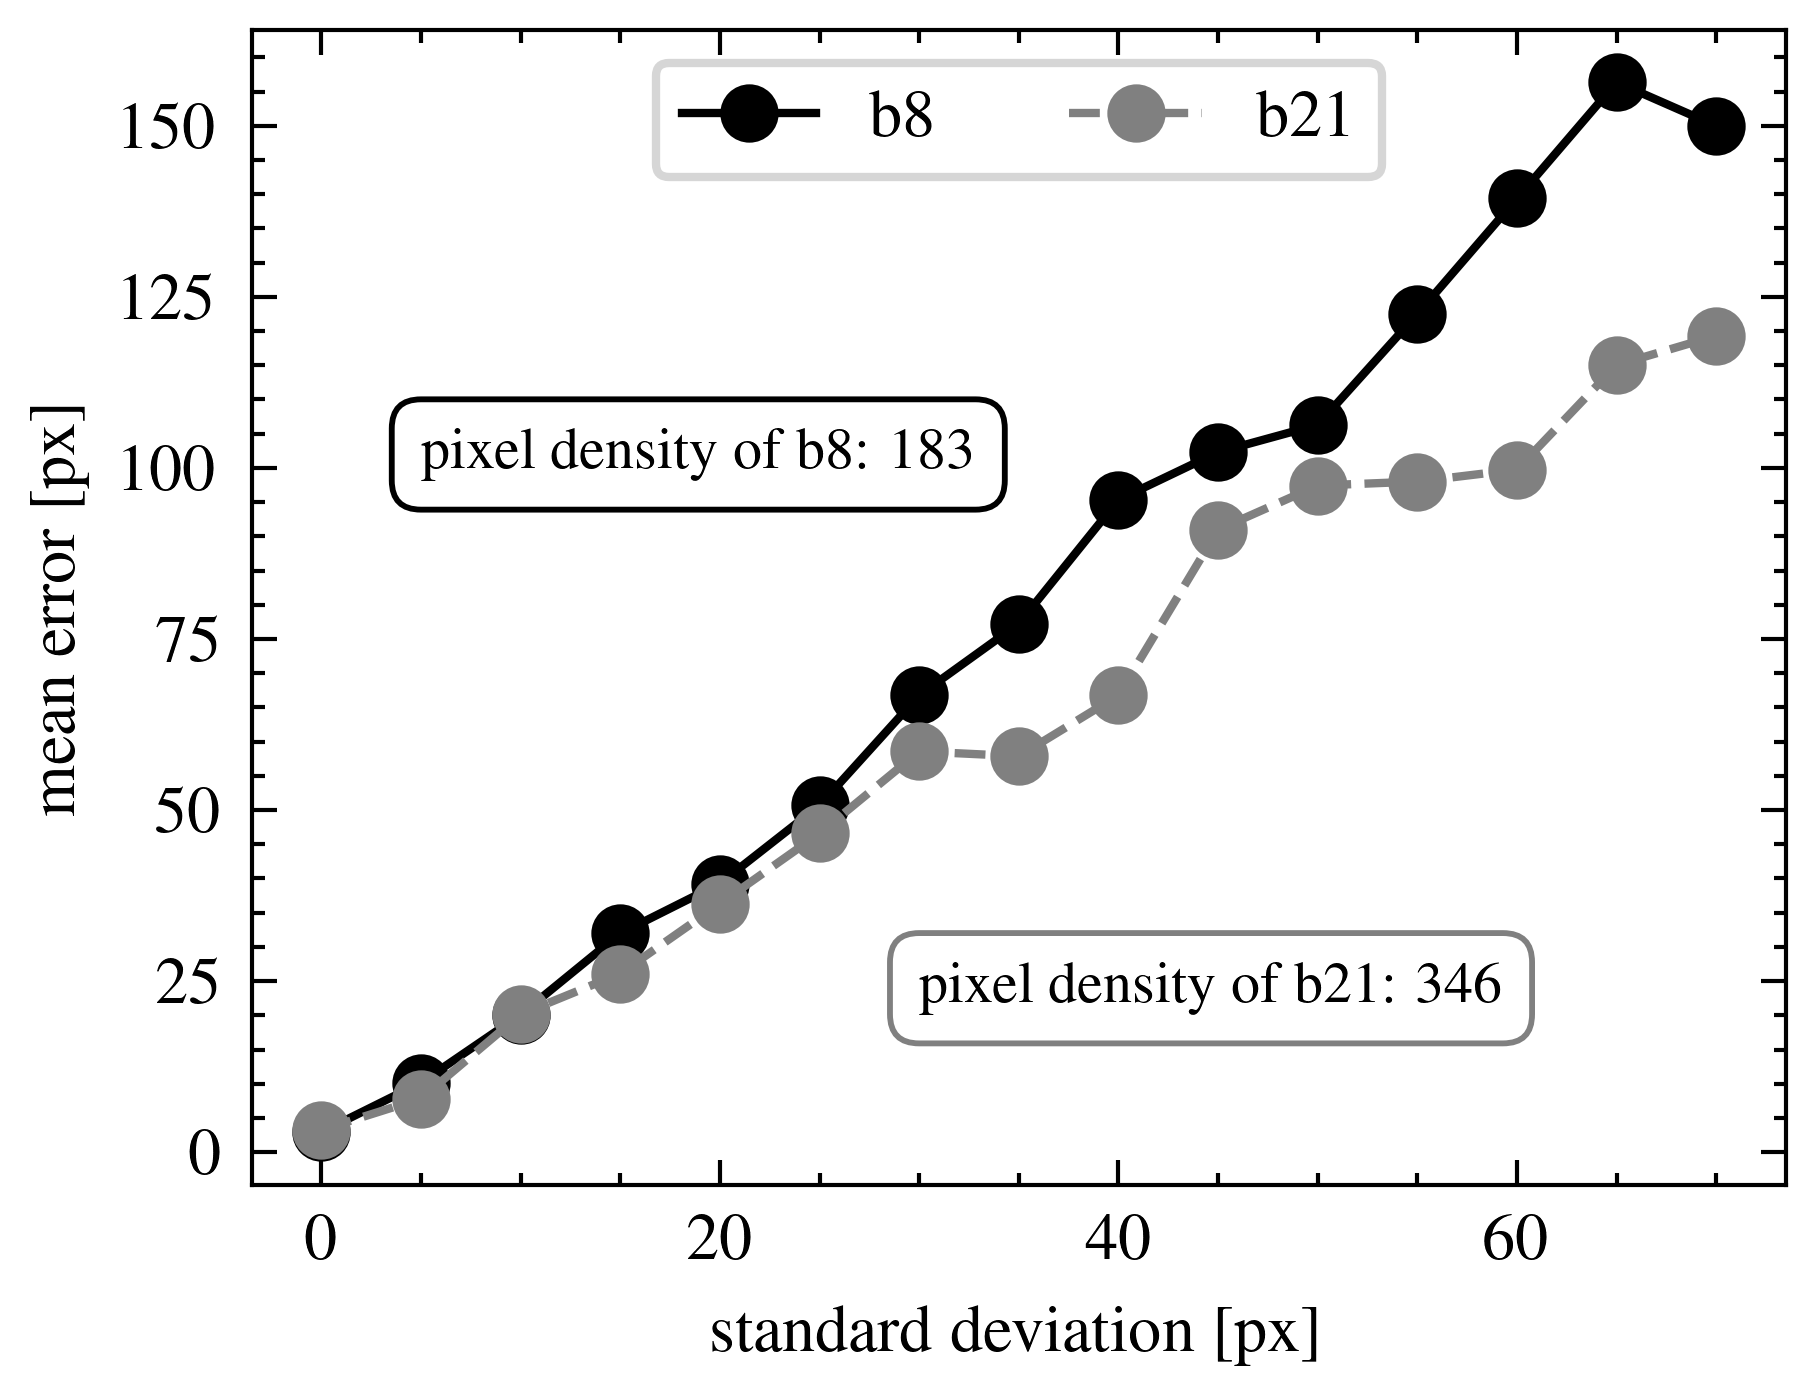
\includegraphics[width=0.40\textwidth]{figures/pixel_density_0026.png}
        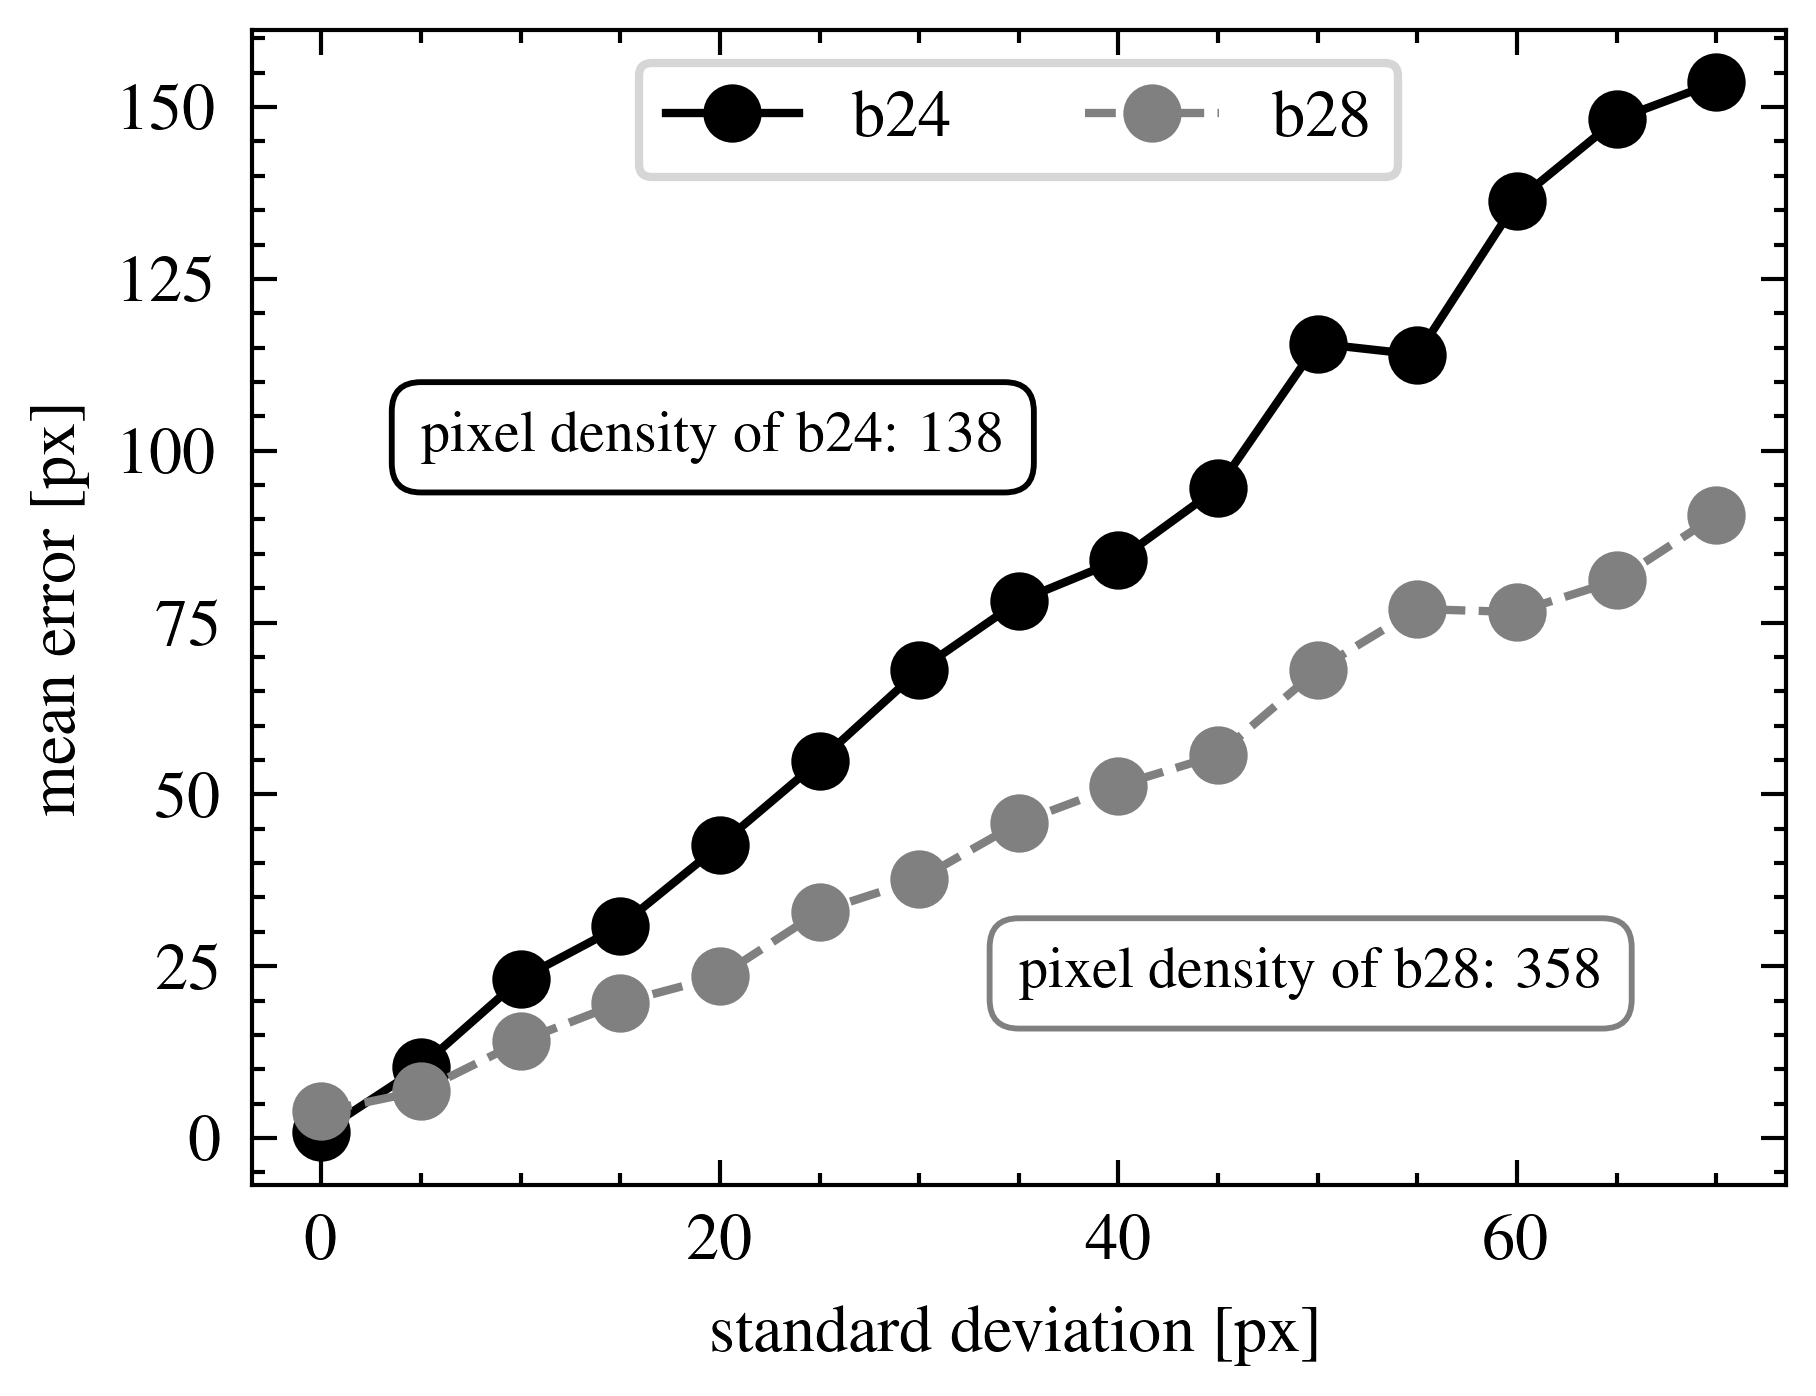
\includegraphics[width=0.40\textwidth]{figures/pixel_density_0029.png}
	\caption{The error for two similar points with different pixel densities 
		while increasing the random Gaussian noise around the reference 
		points, simulating measuring errors.}
	\label{fig:density}
\end{figure}
